\subsection{HTB02 - Time}
<<<<<<< HEAD
    \subsubsection{Escaneo}
        \large{Como inicio de la prueba de penetración se realiza un escaneo de puertos con la herramienta "Nmap", donde se encuentran dos puertos abiertos, el 22 con el servicio SSH y el 80 con un servidor web Apache.}
        \par
        \begin{figure}[h!]
            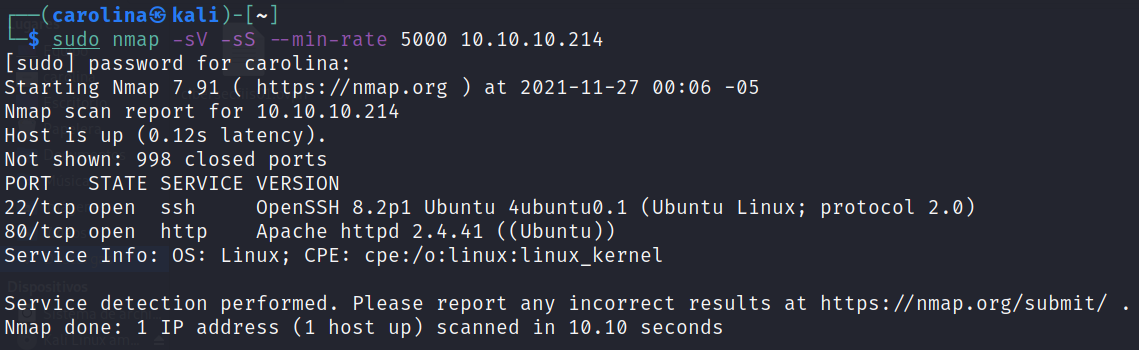
\includegraphics[width=1\textwidth]{imagenes/nmap_time.png} \par \vspace{0.1cm}
            \caption{Escaneo de puertos Time} 
        \end{figure}
    \subsubsection{Análisis de vulnerabilidades y debilidades}
=======
\subsubsection{Escaneo}
\subsubsection{Análisis de Vulnerabilidades}
\subsubsection{Explotación}
\subsubsection{Escalamiento de Privilegios}
\subsubsection{Post-Explotación}
\subsubsection{Recomendaciones de Mitigación}
>>>>>>> f256170ae101aa73e4bc71b5936e56a5d6c15ea0
